% SOURCE: RG_map_evidence_REFIX20260801.json :: cells.*.per_g.{2,3,5,10,20}.{c2_coherent,non_negligible,saturated} per seed; cells ordered by gain
% !TEX encoding = UTF-8 Unicode
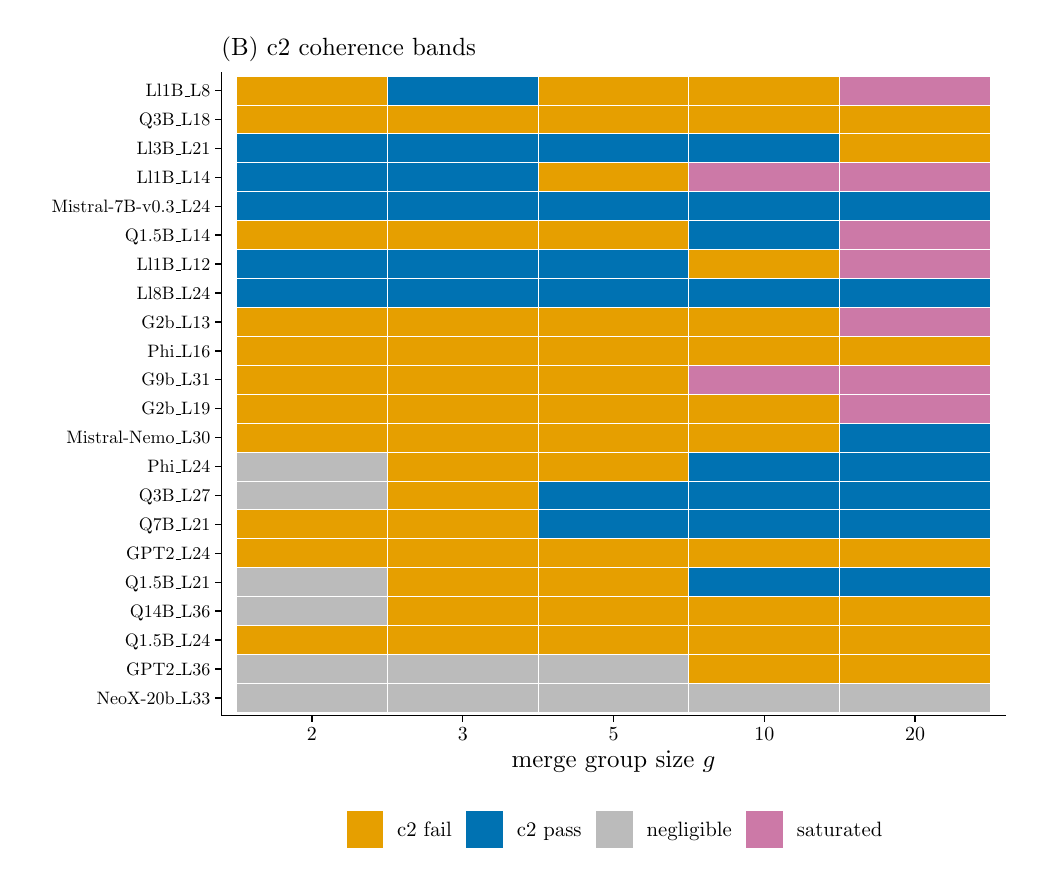
\begin{tikzpicture}[x=1pt,y=1pt]
\definecolor{fillColor}{RGB}{255,255,255}
\path[use as bounding box,fill=fillColor,fill opacity=0.00] (0,0) rectangle (361.35,303.53);
\begin{scope}
\path[clip] (  0.00,  0.00) rectangle (361.35,303.53);
\definecolor{drawColor}{RGB}{255,255,255}
\definecolor{fillColor}{RGB}{255,255,255}

\path[draw=drawColor,line width= 0.5pt,line join=round,line cap=round,fill=fillColor] (  0.00,  0.00) rectangle (361.35,303.53);
\end{scope}
\begin{scope}
\path[clip] ( 70.03, 55.06) rectangle (353.35,287.09);
\definecolor{fillColor}{RGB}{255,255,255}

\path[fill=fillColor] ( 70.03, 55.06) rectangle (353.35,287.09);
\definecolor{drawColor}{RGB}{255,255,255}
\definecolor{fillColor}{RGB}{0,114,178}

\path[draw=drawColor,line width= 0.3pt,fill=fillColor] ( 75.48,202.43) rectangle (129.97,212.88);

\path[draw=drawColor,line width= 0.3pt,fill=fillColor] (129.97,202.43) rectangle (184.45,212.88);

\path[draw=drawColor,line width= 0.3pt,fill=fillColor] (184.45,202.43) rectangle (238.93,212.88);

\path[draw=drawColor,line width= 0.3pt,fill=fillColor] (238.93,202.43) rectangle (293.42,212.88);

\path[draw=drawColor,line width= 0.3pt,fill=fillColor] (293.42,202.43) rectangle (347.90,212.88);

\path[draw=drawColor,line width= 0.3pt,fill=fillColor] ( 75.48,212.88) rectangle (129.97,223.33);

\path[draw=drawColor,line width= 0.3pt,fill=fillColor] (129.97,212.88) rectangle (184.45,223.33);

\path[draw=drawColor,line width= 0.3pt,fill=fillColor] (184.45,212.88) rectangle (238.93,223.33);
\definecolor{fillColor}{RGB}{230,159,0}

\path[draw=drawColor,line width= 0.3pt,fill=fillColor] (238.93,212.88) rectangle (293.42,223.33);
\definecolor{fillColor}{RGB}{204,121,167}

\path[draw=drawColor,line width= 0.3pt,fill=fillColor] (293.42,212.88) rectangle (347.90,223.33);
\definecolor{fillColor}{RGB}{0,114,178}

\path[draw=drawColor,line width= 0.3pt,fill=fillColor] ( 75.48,244.23) rectangle (129.97,254.69);

\path[draw=drawColor,line width= 0.3pt,fill=fillColor] (129.97,244.23) rectangle (184.45,254.69);
\definecolor{fillColor}{RGB}{230,159,0}

\path[draw=drawColor,line width= 0.3pt,fill=fillColor] (184.45,244.23) rectangle (238.93,254.69);
\definecolor{fillColor}{RGB}{204,121,167}

\path[draw=drawColor,line width= 0.3pt,fill=fillColor] (238.93,244.23) rectangle (293.42,254.69);

\path[draw=drawColor,line width= 0.3pt,fill=fillColor] (293.42,244.23) rectangle (347.90,254.69);
\definecolor{fillColor}{RGB}{230,159,0}

\path[draw=drawColor,line width= 0.3pt,fill=fillColor] ( 75.48,275.59) rectangle (129.97,286.04);
\definecolor{fillColor}{RGB}{0,114,178}

\path[draw=drawColor,line width= 0.3pt,fill=fillColor] (129.97,275.59) rectangle (184.45,286.04);
\definecolor{fillColor}{RGB}{230,159,0}

\path[draw=drawColor,line width= 0.3pt,fill=fillColor] (184.45,275.59) rectangle (238.93,286.04);

\path[draw=drawColor,line width= 0.3pt,fill=fillColor] (238.93,275.59) rectangle (293.42,286.04);
\definecolor{fillColor}{RGB}{204,121,167}

\path[draw=drawColor,line width= 0.3pt,fill=fillColor] (293.42,275.59) rectangle (347.90,286.04);
\definecolor{fillColor}{RGB}{0,114,178}

\path[draw=drawColor,line width= 0.3pt,fill=fillColor] ( 75.48,254.69) rectangle (129.97,265.14);

\path[draw=drawColor,line width= 0.3pt,fill=fillColor] (129.97,254.69) rectangle (184.45,265.14);

\path[draw=drawColor,line width= 0.3pt,fill=fillColor] (184.45,254.69) rectangle (238.93,265.14);

\path[draw=drawColor,line width= 0.3pt,fill=fillColor] (238.93,254.69) rectangle (293.42,265.14);
\definecolor{fillColor}{RGB}{230,159,0}

\path[draw=drawColor,line width= 0.3pt,fill=fillColor] (293.42,254.69) rectangle (347.90,265.14);
\definecolor{fillColor}{RGB}{0,114,178}

\path[draw=drawColor,line width= 0.3pt,fill=fillColor] ( 75.48,233.78) rectangle (129.97,244.23);

\path[draw=drawColor,line width= 0.3pt,fill=fillColor] (129.97,233.78) rectangle (184.45,244.23);

\path[draw=drawColor,line width= 0.3pt,fill=fillColor] (184.45,233.78) rectangle (238.93,244.23);

\path[draw=drawColor,line width= 0.3pt,fill=fillColor] (238.93,233.78) rectangle (293.42,244.23);

\path[draw=drawColor,line width= 0.3pt,fill=fillColor] (293.42,233.78) rectangle (347.90,244.23);
\definecolor{fillColor}{RGB}{230,159,0}

\path[draw=drawColor,line width= 0.3pt,fill=fillColor] ( 75.48,150.17) rectangle (129.97,160.62);

\path[draw=drawColor,line width= 0.3pt,fill=fillColor] (129.97,150.17) rectangle (184.45,160.62);

\path[draw=drawColor,line width= 0.3pt,fill=fillColor] (184.45,150.17) rectangle (238.93,160.62);

\path[draw=drawColor,line width= 0.3pt,fill=fillColor] (238.93,150.17) rectangle (293.42,160.62);
\definecolor{fillColor}{RGB}{0,114,178}

\path[draw=drawColor,line width= 0.3pt,fill=fillColor] (293.42,150.17) rectangle (347.90,160.62);
\definecolor{fillColor}{RGB}{230,159,0}

\path[draw=drawColor,line width= 0.3pt,fill=fillColor] ( 75.48,181.52) rectangle (129.97,191.98);

\path[draw=drawColor,line width= 0.3pt,fill=fillColor] (129.97,181.52) rectangle (184.45,191.98);

\path[draw=drawColor,line width= 0.3pt,fill=fillColor] (184.45,181.52) rectangle (238.93,191.98);

\path[draw=drawColor,line width= 0.3pt,fill=fillColor] (238.93,181.52) rectangle (293.42,191.98);

\path[draw=drawColor,line width= 0.3pt,fill=fillColor] (293.42,181.52) rectangle (347.90,191.98);
\definecolor{fillColor}{RGB}{187,187,187}

\path[draw=drawColor,line width= 0.3pt,fill=fillColor] ( 75.48,139.72) rectangle (129.97,150.17);
\definecolor{fillColor}{RGB}{230,159,0}

\path[draw=drawColor,line width= 0.3pt,fill=fillColor] (129.97,139.72) rectangle (184.45,150.17);

\path[draw=drawColor,line width= 0.3pt,fill=fillColor] (184.45,139.72) rectangle (238.93,150.17);
\definecolor{fillColor}{RGB}{0,114,178}

\path[draw=drawColor,line width= 0.3pt,fill=fillColor] (238.93,139.72) rectangle (293.42,150.17);

\path[draw=drawColor,line width= 0.3pt,fill=fillColor] (293.42,139.72) rectangle (347.90,150.17);
\definecolor{fillColor}{RGB}{230,159,0}

\path[draw=drawColor,line width= 0.3pt,fill=fillColor] ( 75.48,223.33) rectangle (129.97,233.78);

\path[draw=drawColor,line width= 0.3pt,fill=fillColor] (129.97,223.33) rectangle (184.45,233.78);

\path[draw=drawColor,line width= 0.3pt,fill=fillColor] (184.45,223.33) rectangle (238.93,233.78);
\definecolor{fillColor}{RGB}{0,114,178}

\path[draw=drawColor,line width= 0.3pt,fill=fillColor] (238.93,223.33) rectangle (293.42,233.78);
\definecolor{fillColor}{RGB}{204,121,167}

\path[draw=drawColor,line width= 0.3pt,fill=fillColor] (293.42,223.33) rectangle (347.90,233.78);
\definecolor{fillColor}{RGB}{187,187,187}

\path[draw=drawColor,line width= 0.3pt,fill=fillColor] ( 75.48, 97.91) rectangle (129.97,108.36);
\definecolor{fillColor}{RGB}{230,159,0}

\path[draw=drawColor,line width= 0.3pt,fill=fillColor] (129.97, 97.91) rectangle (184.45,108.36);

\path[draw=drawColor,line width= 0.3pt,fill=fillColor] (184.45, 97.91) rectangle (238.93,108.36);
\definecolor{fillColor}{RGB}{0,114,178}

\path[draw=drawColor,line width= 0.3pt,fill=fillColor] (238.93, 97.91) rectangle (293.42,108.36);

\path[draw=drawColor,line width= 0.3pt,fill=fillColor] (293.42, 97.91) rectangle (347.90,108.36);
\definecolor{fillColor}{RGB}{230,159,0}

\path[draw=drawColor,line width= 0.3pt,fill=fillColor] ( 75.48, 77.01) rectangle (129.97, 87.46);

\path[draw=drawColor,line width= 0.3pt,fill=fillColor] (129.97, 77.01) rectangle (184.45, 87.46);

\path[draw=drawColor,line width= 0.3pt,fill=fillColor] (184.45, 77.01) rectangle (238.93, 87.46);

\path[draw=drawColor,line width= 0.3pt,fill=fillColor] (238.93, 77.01) rectangle (293.42, 87.46);

\path[draw=drawColor,line width= 0.3pt,fill=fillColor] (293.42, 77.01) rectangle (347.90, 87.46);
\definecolor{fillColor}{RGB}{187,187,187}

\path[draw=drawColor,line width= 0.3pt,fill=fillColor] ( 75.48, 87.46) rectangle (129.97, 97.91);
\definecolor{fillColor}{RGB}{230,159,0}

\path[draw=drawColor,line width= 0.3pt,fill=fillColor] (129.97, 87.46) rectangle (184.45, 97.91);

\path[draw=drawColor,line width= 0.3pt,fill=fillColor] (184.45, 87.46) rectangle (238.93, 97.91);

\path[draw=drawColor,line width= 0.3pt,fill=fillColor] (238.93, 87.46) rectangle (293.42, 97.91);

\path[draw=drawColor,line width= 0.3pt,fill=fillColor] (293.42, 87.46) rectangle (347.90, 97.91);

\path[draw=drawColor,line width= 0.3pt,fill=fillColor] ( 75.48,265.14) rectangle (129.97,275.59);

\path[draw=drawColor,line width= 0.3pt,fill=fillColor] (129.97,265.14) rectangle (184.45,275.59);

\path[draw=drawColor,line width= 0.3pt,fill=fillColor] (184.45,265.14) rectangle (238.93,275.59);

\path[draw=drawColor,line width= 0.3pt,fill=fillColor] (238.93,265.14) rectangle (293.42,275.59);

\path[draw=drawColor,line width= 0.3pt,fill=fillColor] (293.42,265.14) rectangle (347.90,275.59);
\definecolor{fillColor}{RGB}{187,187,187}

\path[draw=drawColor,line width= 0.3pt,fill=fillColor] ( 75.48,129.27) rectangle (129.97,139.72);
\definecolor{fillColor}{RGB}{230,159,0}

\path[draw=drawColor,line width= 0.3pt,fill=fillColor] (129.97,129.27) rectangle (184.45,139.72);
\definecolor{fillColor}{RGB}{0,114,178}

\path[draw=drawColor,line width= 0.3pt,fill=fillColor] (184.45,129.27) rectangle (238.93,139.72);

\path[draw=drawColor,line width= 0.3pt,fill=fillColor] (238.93,129.27) rectangle (293.42,139.72);

\path[draw=drawColor,line width= 0.3pt,fill=fillColor] (293.42,129.27) rectangle (347.90,139.72);
\definecolor{fillColor}{RGB}{230,159,0}

\path[draw=drawColor,line width= 0.3pt,fill=fillColor] ( 75.48,118.82) rectangle (129.97,129.27);

\path[draw=drawColor,line width= 0.3pt,fill=fillColor] (129.97,118.82) rectangle (184.45,129.27);
\definecolor{fillColor}{RGB}{0,114,178}

\path[draw=drawColor,line width= 0.3pt,fill=fillColor] (184.45,118.82) rectangle (238.93,129.27);

\path[draw=drawColor,line width= 0.3pt,fill=fillColor] (238.93,118.82) rectangle (293.42,129.27);

\path[draw=drawColor,line width= 0.3pt,fill=fillColor] (293.42,118.82) rectangle (347.90,129.27);
\definecolor{fillColor}{RGB}{230,159,0}

\path[draw=drawColor,line width= 0.3pt,fill=fillColor] ( 75.48,191.98) rectangle (129.97,202.43);

\path[draw=drawColor,line width= 0.3pt,fill=fillColor] (129.97,191.98) rectangle (184.45,202.43);

\path[draw=drawColor,line width= 0.3pt,fill=fillColor] (184.45,191.98) rectangle (238.93,202.43);

\path[draw=drawColor,line width= 0.3pt,fill=fillColor] (238.93,191.98) rectangle (293.42,202.43);
\definecolor{fillColor}{RGB}{204,121,167}

\path[draw=drawColor,line width= 0.3pt,fill=fillColor] (293.42,191.98) rectangle (347.90,202.43);
\definecolor{fillColor}{RGB}{230,159,0}

\path[draw=drawColor,line width= 0.3pt,fill=fillColor] ( 75.48,160.62) rectangle (129.97,171.07);

\path[draw=drawColor,line width= 0.3pt,fill=fillColor] (129.97,160.62) rectangle (184.45,171.07);

\path[draw=drawColor,line width= 0.3pt,fill=fillColor] (184.45,160.62) rectangle (238.93,171.07);

\path[draw=drawColor,line width= 0.3pt,fill=fillColor] (238.93,160.62) rectangle (293.42,171.07);
\definecolor{fillColor}{RGB}{204,121,167}

\path[draw=drawColor,line width= 0.3pt,fill=fillColor] (293.42,160.62) rectangle (347.90,171.07);
\definecolor{fillColor}{RGB}{230,159,0}

\path[draw=drawColor,line width= 0.3pt,fill=fillColor] ( 75.48,171.07) rectangle (129.97,181.52);

\path[draw=drawColor,line width= 0.3pt,fill=fillColor] (129.97,171.07) rectangle (184.45,181.52);

\path[draw=drawColor,line width= 0.3pt,fill=fillColor] (184.45,171.07) rectangle (238.93,181.52);
\definecolor{fillColor}{RGB}{204,121,167}

\path[draw=drawColor,line width= 0.3pt,fill=fillColor] (238.93,171.07) rectangle (293.42,181.52);

\path[draw=drawColor,line width= 0.3pt,fill=fillColor] (293.42,171.07) rectangle (347.90,181.52);
\definecolor{fillColor}{RGB}{187,187,187}

\path[draw=drawColor,line width= 0.3pt,fill=fillColor] ( 75.48, 56.11) rectangle (129.97, 66.56);

\path[draw=drawColor,line width= 0.3pt,fill=fillColor] (129.97, 56.11) rectangle (184.45, 66.56);

\path[draw=drawColor,line width= 0.3pt,fill=fillColor] (184.45, 56.11) rectangle (238.93, 66.56);

\path[draw=drawColor,line width= 0.3pt,fill=fillColor] (238.93, 56.11) rectangle (293.42, 66.56);

\path[draw=drawColor,line width= 0.3pt,fill=fillColor] (293.42, 56.11) rectangle (347.90, 66.56);
\definecolor{fillColor}{RGB}{230,159,0}

\path[draw=drawColor,line width= 0.3pt,fill=fillColor] ( 75.48,108.36) rectangle (129.97,118.82);

\path[draw=drawColor,line width= 0.3pt,fill=fillColor] (129.97,108.36) rectangle (184.45,118.82);

\path[draw=drawColor,line width= 0.3pt,fill=fillColor] (184.45,108.36) rectangle (238.93,118.82);

\path[draw=drawColor,line width= 0.3pt,fill=fillColor] (238.93,108.36) rectangle (293.42,118.82);

\path[draw=drawColor,line width= 0.3pt,fill=fillColor] (293.42,108.36) rectangle (347.90,118.82);
\definecolor{fillColor}{RGB}{187,187,187}

\path[draw=drawColor,line width= 0.3pt,fill=fillColor] ( 75.48, 66.56) rectangle (129.97, 77.01);

\path[draw=drawColor,line width= 0.3pt,fill=fillColor] (129.97, 66.56) rectangle (184.45, 77.01);

\path[draw=drawColor,line width= 0.3pt,fill=fillColor] (184.45, 66.56) rectangle (238.93, 77.01);
\definecolor{fillColor}{RGB}{230,159,0}

\path[draw=drawColor,line width= 0.3pt,fill=fillColor] (238.93, 66.56) rectangle (293.42, 77.01);

\path[draw=drawColor,line width= 0.3pt,fill=fillColor] (293.42, 66.56) rectangle (347.90, 77.01);
\end{scope}
\begin{scope}
\path[clip] (  0.00,  0.00) rectangle (361.35,303.53);
\definecolor{drawColor}{RGB}{0,0,0}

\path[draw=drawColor,line width= 0.5pt,line join=round,line cap=rect] ( 70.03, 55.06) --
	( 70.03,287.09);
\end{scope}
\begin{scope}
\path[clip] (  0.00,  0.00) rectangle (361.35,303.53);
\definecolor{drawColor}{RGB}{0,0,0}

\node[text=drawColor,anchor=base east,inner sep=0pt, outer sep=0pt, scale=  0.65] at ( 65.98, 59.09) {NeoX-20b\_L33};

\node[text=drawColor,anchor=base east,inner sep=0pt, outer sep=0pt, scale=  0.65] at ( 65.98, 69.54) {GPT2\_L36};

\node[text=drawColor,anchor=base east,inner sep=0pt, outer sep=0pt, scale=  0.65] at ( 65.98, 80.00) {Q1.5B\_L24};

\node[text=drawColor,anchor=base east,inner sep=0pt, outer sep=0pt, scale=  0.65] at ( 65.98, 90.45) {Q14B\_L36};

\node[text=drawColor,anchor=base east,inner sep=0pt, outer sep=0pt, scale=  0.65] at ( 65.98,100.90) {Q1.5B\_L21};

\node[text=drawColor,anchor=base east,inner sep=0pt, outer sep=0pt, scale=  0.65] at ( 65.98,111.35) {GPT2\_L24};

\node[text=drawColor,anchor=base east,inner sep=0pt, outer sep=0pt, scale=  0.65] at ( 65.98,121.80) {Q7B\_L21};

\node[text=drawColor,anchor=base east,inner sep=0pt, outer sep=0pt, scale=  0.65] at ( 65.98,132.25) {Q3B\_L27};

\node[text=drawColor,anchor=base east,inner sep=0pt, outer sep=0pt, scale=  0.65] at ( 65.98,142.71) {Phi\_L24};

\node[text=drawColor,anchor=base east,inner sep=0pt, outer sep=0pt, scale=  0.65] at ( 65.98,153.16) {Mistral-Nemo\_L30};

\node[text=drawColor,anchor=base east,inner sep=0pt, outer sep=0pt, scale=  0.65] at ( 65.98,163.61) {G2b\_L19};

\node[text=drawColor,anchor=base east,inner sep=0pt, outer sep=0pt, scale=  0.65] at ( 65.98,174.06) {G9b\_L31};

\node[text=drawColor,anchor=base east,inner sep=0pt, outer sep=0pt, scale=  0.65] at ( 65.98,184.51) {Phi\_L16};

\node[text=drawColor,anchor=base east,inner sep=0pt, outer sep=0pt, scale=  0.65] at ( 65.98,194.96) {G2b\_L13};

\node[text=drawColor,anchor=base east,inner sep=0pt, outer sep=0pt, scale=  0.65] at ( 65.98,205.42) {Ll8B\_L24};

\node[text=drawColor,anchor=base east,inner sep=0pt, outer sep=0pt, scale=  0.65] at ( 65.98,215.87) {Ll1B\_L12};

\node[text=drawColor,anchor=base east,inner sep=0pt, outer sep=0pt, scale=  0.65] at ( 65.98,226.32) {Q1.5B\_L14};

\node[text=drawColor,anchor=base east,inner sep=0pt, outer sep=0pt, scale=  0.65] at ( 65.98,236.77) {Mistral-7B-v0.3\_L24};

\node[text=drawColor,anchor=base east,inner sep=0pt, outer sep=0pt, scale=  0.65] at ( 65.98,247.22) {Ll1B\_L14};

\node[text=drawColor,anchor=base east,inner sep=0pt, outer sep=0pt, scale=  0.65] at ( 65.98,257.67) {Ll3B\_L21};

\node[text=drawColor,anchor=base east,inner sep=0pt, outer sep=0pt, scale=  0.65] at ( 65.98,268.13) {Q3B\_L18};

\node[text=drawColor,anchor=base east,inner sep=0pt, outer sep=0pt, scale=  0.65] at ( 65.98,278.58) {Ll1B\_L8};
\end{scope}
\begin{scope}
\path[clip] (  0.00,  0.00) rectangle (361.35,303.53);
\definecolor{drawColor}{RGB}{0,0,0}

\path[draw=drawColor,line width= 0.5pt,line join=round] ( 67.78, 61.33) --
	( 70.03, 61.33);

\path[draw=drawColor,line width= 0.5pt,line join=round] ( 67.78, 71.78) --
	( 70.03, 71.78);

\path[draw=drawColor,line width= 0.5pt,line join=round] ( 67.78, 82.23) --
	( 70.03, 82.23);

\path[draw=drawColor,line width= 0.5pt,line join=round] ( 67.78, 92.69) --
	( 70.03, 92.69);

\path[draw=drawColor,line width= 0.5pt,line join=round] ( 67.78,103.14) --
	( 70.03,103.14);

\path[draw=drawColor,line width= 0.5pt,line join=round] ( 67.78,113.59) --
	( 70.03,113.59);

\path[draw=drawColor,line width= 0.5pt,line join=round] ( 67.78,124.04) --
	( 70.03,124.04);

\path[draw=drawColor,line width= 0.5pt,line join=round] ( 67.78,134.49) --
	( 70.03,134.49);

\path[draw=drawColor,line width= 0.5pt,line join=round] ( 67.78,144.94) --
	( 70.03,144.94);

\path[draw=drawColor,line width= 0.5pt,line join=round] ( 67.78,155.40) --
	( 70.03,155.40);

\path[draw=drawColor,line width= 0.5pt,line join=round] ( 67.78,165.85) --
	( 70.03,165.85);

\path[draw=drawColor,line width= 0.5pt,line join=round] ( 67.78,176.30) --
	( 70.03,176.30);

\path[draw=drawColor,line width= 0.5pt,line join=round] ( 67.78,186.75) --
	( 70.03,186.75);

\path[draw=drawColor,line width= 0.5pt,line join=round] ( 67.78,197.20) --
	( 70.03,197.20);

\path[draw=drawColor,line width= 0.5pt,line join=round] ( 67.78,207.65) --
	( 70.03,207.65);

\path[draw=drawColor,line width= 0.5pt,line join=round] ( 67.78,218.11) --
	( 70.03,218.11);

\path[draw=drawColor,line width= 0.5pt,line join=round] ( 67.78,228.56) --
	( 70.03,228.56);

\path[draw=drawColor,line width= 0.5pt,line join=round] ( 67.78,239.01) --
	( 70.03,239.01);

\path[draw=drawColor,line width= 0.5pt,line join=round] ( 67.78,249.46) --
	( 70.03,249.46);

\path[draw=drawColor,line width= 0.5pt,line join=round] ( 67.78,259.91) --
	( 70.03,259.91);

\path[draw=drawColor,line width= 0.5pt,line join=round] ( 67.78,270.36) --
	( 70.03,270.36);

\path[draw=drawColor,line width= 0.5pt,line join=round] ( 67.78,280.82) --
	( 70.03,280.82);
\end{scope}
\begin{scope}
\path[clip] (  0.00,  0.00) rectangle (361.35,303.53);
\definecolor{drawColor}{RGB}{0,0,0}

\path[draw=drawColor,line width= 0.5pt,line join=round,line cap=rect] ( 70.03, 55.06) --
	(353.35, 55.06);
\end{scope}
\begin{scope}
\path[clip] (  0.00,  0.00) rectangle (361.35,303.53);
\definecolor{drawColor}{RGB}{0,0,0}

\path[draw=drawColor,line width= 0.5pt,line join=round] (102.72, 52.81) --
	(102.72, 55.06);

\path[draw=drawColor,line width= 0.5pt,line join=round] (157.21, 52.81) --
	(157.21, 55.06);

\path[draw=drawColor,line width= 0.5pt,line join=round] (211.69, 52.81) --
	(211.69, 55.06);

\path[draw=drawColor,line width= 0.5pt,line join=round] (266.18, 52.81) --
	(266.18, 55.06);

\path[draw=drawColor,line width= 0.5pt,line join=round] (320.66, 52.81) --
	(320.66, 55.06);
\end{scope}
\begin{scope}
\path[clip] (  0.00,  0.00) rectangle (361.35,303.53);
\definecolor{drawColor}{RGB}{0,0,0}

\node[text=drawColor,anchor=base,inner sep=0pt, outer sep=0pt, scale=  0.72] at (102.72, 46.05) {2};

\node[text=drawColor,anchor=base,inner sep=0pt, outer sep=0pt, scale=  0.72] at (157.21, 46.05) {3};

\node[text=drawColor,anchor=base,inner sep=0pt, outer sep=0pt, scale=  0.72] at (211.69, 46.05) {5};

\node[text=drawColor,anchor=base,inner sep=0pt, outer sep=0pt, scale=  0.72] at (266.18, 46.05) {10};

\node[text=drawColor,anchor=base,inner sep=0pt, outer sep=0pt, scale=  0.72] at (320.66, 46.05) {20};
\end{scope}
\begin{scope}
\path[clip] (  0.00,  0.00) rectangle (361.35,303.53);
\definecolor{drawColor}{RGB}{0,0,0}

\node[text=drawColor,anchor=base,inner sep=0pt, outer sep=0pt, scale=  0.90] at (211.69, 36.20) {merge group size $g$};
\end{scope}
\begin{scope}
\path[clip] (  0.00,  0.00) rectangle (361.35,303.53);
\definecolor{fillColor}{RGB}{255,255,255}

\path[fill=fillColor] (110.08,  2.00) rectangle (313.31, 25.45);
\end{scope}
\begin{scope}
\path[clip] (  0.00,  0.00) rectangle (361.35,303.53);
\definecolor{fillColor}{RGB}{255,255,255}

\path[fill=fillColor] (114.58,  6.50) rectangle (129.03, 20.95);
\definecolor{drawColor}{RGB}{255,255,255}
\definecolor{fillColor}{RGB}{230,159,0}

\path[draw=drawColor,line width= 0.3pt,fill=fillColor] (115.00,  6.93) rectangle (128.60, 20.53);
\end{scope}
\begin{scope}
\path[clip] (  0.00,  0.00) rectangle (361.35,303.53);
\definecolor{fillColor}{RGB}{255,255,255}

\path[fill=fillColor] (157.82,  6.50) rectangle (172.27, 20.95);
\definecolor{drawColor}{RGB}{255,255,255}
\definecolor{fillColor}{RGB}{0,114,178}

\path[draw=drawColor,line width= 0.3pt,fill=fillColor] (158.25,  6.93) rectangle (171.85, 20.53);
\end{scope}
\begin{scope}
\path[clip] (  0.00,  0.00) rectangle (361.35,303.53);
\definecolor{fillColor}{RGB}{255,255,255}

\path[fill=fillColor] (204.68,  6.50) rectangle (219.14, 20.95);
\definecolor{drawColor}{RGB}{255,255,255}
\definecolor{fillColor}{RGB}{187,187,187}

\path[draw=drawColor,line width= 0.3pt,fill=fillColor] (205.11,  6.93) rectangle (218.71, 20.53);
\end{scope}
\begin{scope}
\path[clip] (  0.00,  0.00) rectangle (361.35,303.53);
\definecolor{fillColor}{RGB}{255,255,255}

\path[fill=fillColor] (258.96,  6.50) rectangle (273.42, 20.95);
\definecolor{drawColor}{RGB}{255,255,255}
\definecolor{fillColor}{RGB}{204,121,167}

\path[draw=drawColor,line width= 0.3pt,fill=fillColor] (259.39,  6.93) rectangle (272.99, 20.53);
\end{scope}
\begin{scope}
\path[clip] (  0.00,  0.00) rectangle (361.35,303.53);
\definecolor{drawColor}{RGB}{0,0,0}

\node[text=drawColor,anchor=base west,inner sep=0pt, outer sep=0pt, scale=  0.75] at (133.53, 11.14) {c2 fail};
\end{scope}
\begin{scope}
\path[clip] (  0.00,  0.00) rectangle (361.35,303.53);
\definecolor{drawColor}{RGB}{0,0,0}

\node[text=drawColor,anchor=base west,inner sep=0pt, outer sep=0pt, scale=  0.75] at (176.77, 11.14) {c2 pass};
\end{scope}
\begin{scope}
\path[clip] (  0.00,  0.00) rectangle (361.35,303.53);
\definecolor{drawColor}{RGB}{0,0,0}

\node[text=drawColor,anchor=base west,inner sep=0pt, outer sep=0pt, scale=  0.75] at (223.64, 11.14) {negligible};
\end{scope}
\begin{scope}
\path[clip] (  0.00,  0.00) rectangle (361.35,303.53);
\definecolor{drawColor}{RGB}{0,0,0}

\node[text=drawColor,anchor=base west,inner sep=0pt, outer sep=0pt, scale=  0.75] at (277.92, 11.14) {saturated};
\end{scope}
\begin{scope}
\path[clip] (  0.00,  0.00) rectangle (361.35,303.53);
\definecolor{drawColor}{RGB}{0,0,0}

\node[text=drawColor,anchor=base west,inner sep=0pt, outer sep=0pt, scale=  0.90] at ( 70.03,293.34) {(B) c2 coherence bands};
\end{scope}
\end{tikzpicture}
